\documentclass[12pt]{article}
\usepackage[margin=2.5cm]{geometry}
\usepackage{enumerate}
\usepackage{amsfonts}
\usepackage{amsmath}
\usepackage{fancyhdr}
\usepackage{amsmath}
\usepackage{amssymb}
\usepackage{amsthm}
\usepackage{mdframed}
\usepackage{graphicx}
\usepackage{subcaption}
\usepackage{adjustbox}
\usepackage{listings}
\usepackage{xcolor}
\usepackage{booktabs}
\usepackage[utf]{kotex}
\usepackage{hyperref}

\definecolor{codegreen}{rgb}{0,0.6,0}
\definecolor{codegray}{rgb}{0.5,0.5,0.5}
\definecolor{codepurple}{rgb}{0.58,0,0.82}
\definecolor{backcolour}{rgb}{0.95,0.95,0.92}

\lstdefinestyle{mystyle}{
    backgroundcolor=\color{backcolour},
    commentstyle=\color{codegreen},
    keywordstyle=\color{magenta},
    numberstyle=\tiny\color{codegray},
    stringstyle=\color{codepurple},
    basicstyle=\ttfamily\footnotesize,
    breakatwhitespace=false,
    breaklines=true,
    captionpos=b,
    keepspaces=true,
    numbers=left,
    numbersep=5pt,
    showspaces=false,
    showstringspaces=false,
    showtabs=false,
    tabsize=1
}

\lstset{style=mystyle}

\pagestyle{fancy}
\renewcommand{\headrulewidth}{0.4pt}
\lhead{Hyungmo Gu}
\rhead{CSC369 Week 5 Notes}

\begin{document}
\title{CSC369 Week 5 Notes}
\author{Hyungmo Gu}
\maketitle

\bigskip

\section{Memory Management}

\begin{itemize}
    % \item Recap
    % \item What does real systems do?
    \item Physical Memory vs Virtual Memory $^{[1]}$
    \begin{itemize}
        \item Physical Memory
        \begin{itemize}
            \item Is RAM :)!!
            \item Is the first memory used when computer requires memory such as
            loading application or OS
        \end{itemize}
        \item Virtual Memory
        \begin{itemize}
            \item Is stored on hard drive
            \item Is used when RAM is filled
            \item Is slower than RAM
        \end{itemize}
    \end{itemize}

    \bigskip

    \underline{\textbf{Refernces:}}

    \bigskip

    \begin{enumerate}[1)]
        \item Tech Walla: What Is the Difference Between Virtual Memory \& Physical Memory?, \href{https://www.techwalla.com/articles/difference-virtual-memory-physical-memory_}{link}
    \end{enumerate}

    \item Memory Management
    \begin{itemize}
        \item Is the process of controlling and coordinating computer memory
        \item Assings portions known as \textbf{blocks} to various programs $^{[1]}$
    \end{itemize}

    \underline{\textbf{Refernces:}}

    \bigskip

    \begin{enumerate}[1)]
        \item Guru 99: Memory Management in OS: Contiguous, Swapping, Fragmentation \& Physical Memory?, \href{https://www.guru99.com/os-memory-management.html#1}{link}
    \end{enumerate}
    % \item Requirements
    % \item Meeting the Requirements
    % \item Address Binding
    % \item When are Addresses Bound?
    % \item Load-Time Binding Example
    % \item A better plan
    % \item Memory Management
    % \item Address Translation: Logical and Physical Addresses
    % \item How to Allocate Physical Memory?
    \item Fixed Partitioning
    \begin{itemize}
        \item Is the oldest and simplest technique to put more than one processes in
        the main memory. $^{[1]}$
        \item Divides memory into regions with fixed boundaries.
        \begin{itemize}
            \item Can be of equal size
            \item Or unequal size
        \end{itemize}
        \item Advantages: $^{[1]}$
        \begin{itemize}
            \item Is easy to implement
            \item Requires lesser indirect computational power
        \end{itemize}
        \item Disadvantages: $^{[1]}$
        \begin{itemize}
            \item Creates a gap if process is smaller than partition (\textbf{Internal Fragmentation})
            \item Programmer must deal with programs larger than partition
        \end{itemize}
    \end{itemize}

    \begin{center}
    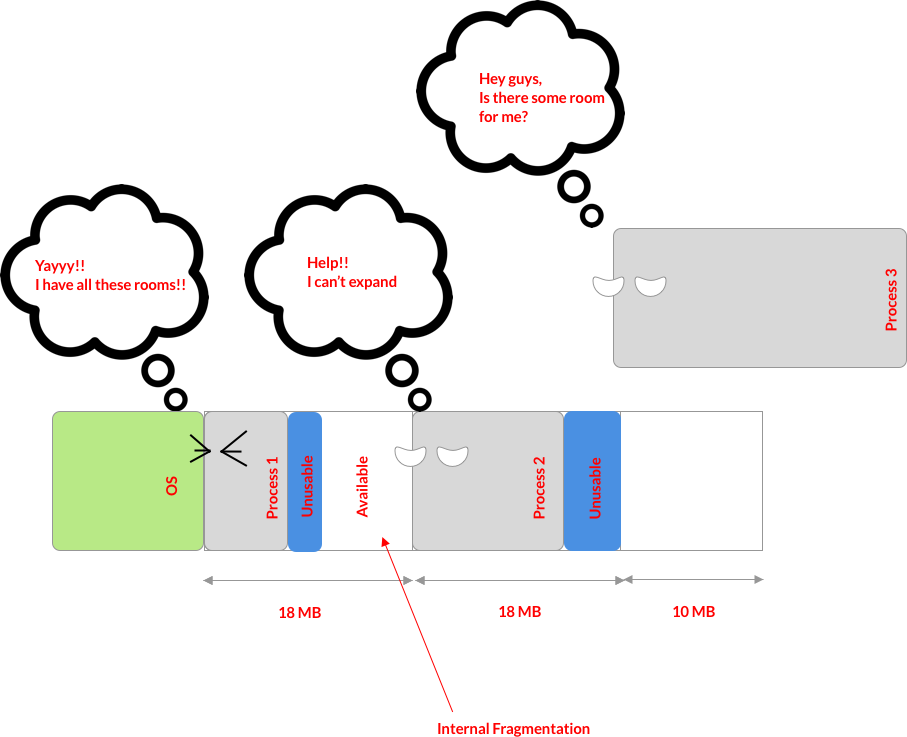
\includegraphics[width=0.8\linewidth]{images/week_5_notes_1_1.png}
    \end{center}

    \bigskip

    \underline{\textbf{Refernces:}}

    \bigskip

    \begin{enumerate}[1)]
        \item Chegg Study: Fixed Partitions, \href{https://www.chegg.com/homework-help/definitions/fixed-partitions-3}{link}
    \end{enumerate}
    % \item Placement with Fixed Partitions
    % \item Placement Example (Queue per Partition)
    \item Dynamic Partitioning
    \begin{itemize}
        \item Allevates problems caused by fixed partitioning $^{[1]}$
        \item A partition of exact the right size is created for a process
        \item OS may move processes around to create larger chunks of space
        \begin{itemize}
            \item I.e. moving process 3 right beneath process 1
            \item Is called \textbf{compaction}
            \item Processes \underline{must} be \textbf{relocatable}
        \end{itemize}

        \begin{center}
        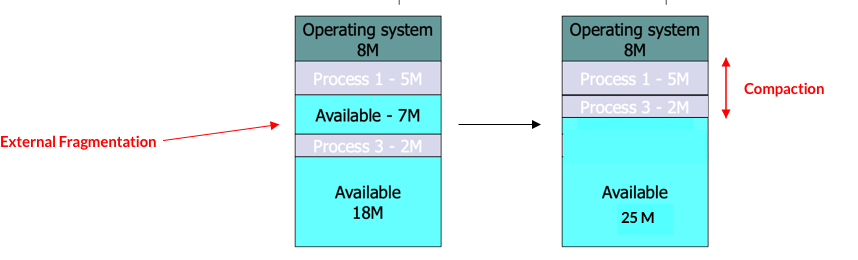
\includegraphics[width=0.8\linewidth]{images/week_5_notes_1_2.png}
        \end{center}

        \item Advantages $^{[1]}$
        \begin{itemize}
            \item No \textbf{internal fragmentation}
            \begin{itemize}
                \item There will be no unused space left in the partition

                \begin{center}
                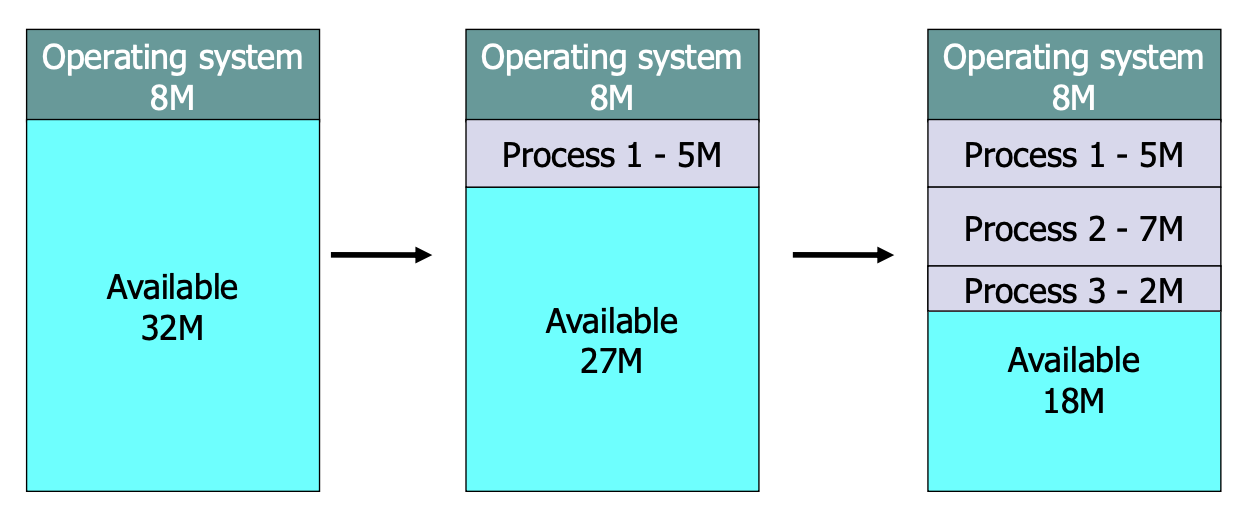
\includegraphics[width=0.7\linewidth]{images/week_5_notes_1_3.png}
                \end{center}
            \end{itemize}
            \item No restriction on degree of multiprogramming $^{[1]}$
            \begin{itemize}
                \item More proccesses in memory due to absence of internal
                fragmentation
                \item Processes can be loaded until RAM is empty
            \end{itemize}
            \item No limitation on the size of process
            \begin{itemize}
                \item Process size not limited to the size of partition
            \end{itemize}
        \end{itemize}
        \item Disadvantages
        \begin{itemize}
            \item As processes come and go `holes' are created
            \begin{itemize}
                \item Is called \textbf{external fragmentation}
            \end{itemize}
        \end{itemize}
    \end{itemize}

    \begin{center}
    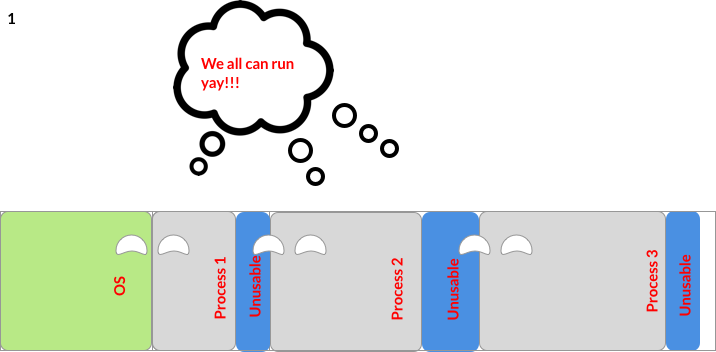
\includegraphics[width=0.8\linewidth]{images/week_5_notes_1_5.png}
    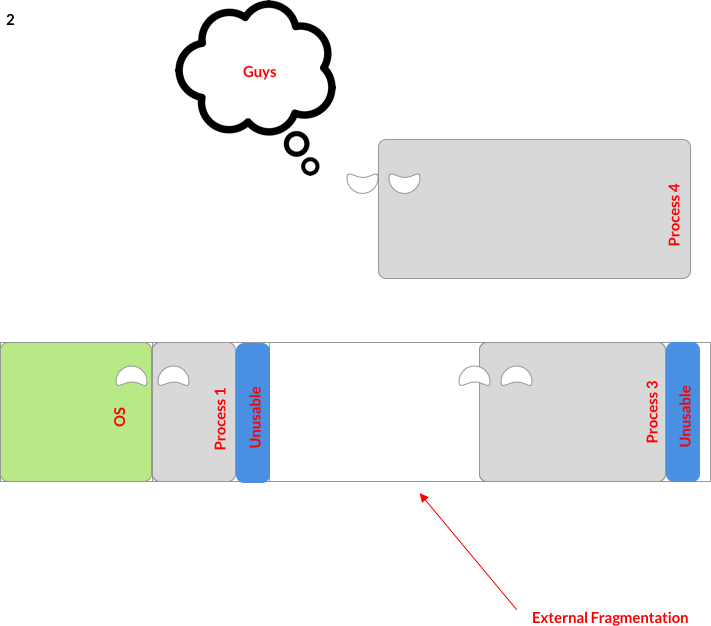
\includegraphics[width=0.8\linewidth]{images/week_5_notes_1_6.png}
    \end{center}

    \underline{\textbf{Refernces:}}

    \bigskip

    \begin{enumerate}[1)]
        \item GeeksForGeeks: Variable (or dynamic) Partitioning in Operating System, \href{https://www.geeksforgeeks.org/variable-or-dynamic-partitioning-in-operating-system/}{link}
    \end{enumerate}
    % \item More Dynamic Partitioning
    % \item Heap Management
    % \item Tracking Memory Allocation
    % \item Freeing Blocks
    % \item Placement Algorithms
    % \item Comparing Placement Algorithms
    % \item Problems with Paging
    \item Paging
    \begin{itemize}
        \item Solves \textbf{internal fragmentation} and \textbf{external fragmentation}
        \item Stores and retrieves data from \textbf{secondary storage} for use
        in \textbf{main memory} $^{[1]}$
        \begin{itemize}
            \item Secondary storage $\to$ Hard Drive
            \item Main memory $\to$ RAM
        \end{itemize}
        \item Is an important part of \textbf{virtual memory} management in modern
        OS $^{[1]}$
        \item Partitions memory into equal, fixed-size chunks
        \begin{itemize}
            \item Are called \textbf{page frames} or \textbf{frames}
        \end{itemize}
        \item Divide processes' memory into chunks of the same size
        \begin{itemize}
            \item These are called \textbf{pages}
        \end{itemize}
    \end{itemize}

    \begin{figure}[h!]
    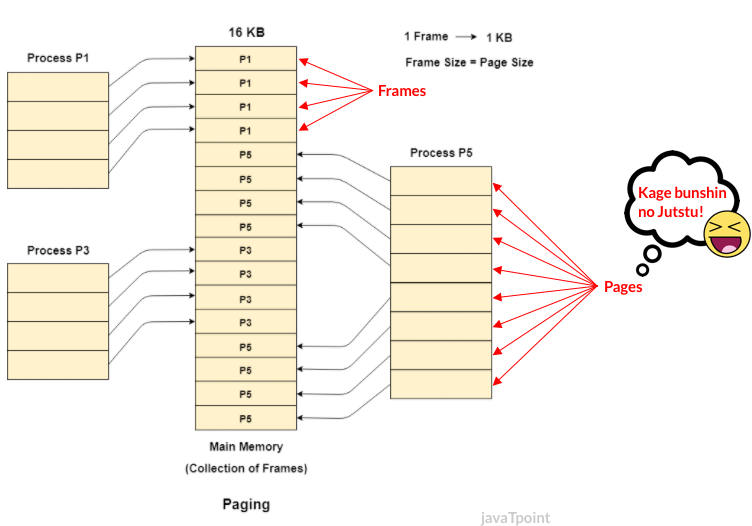
\includegraphics[width=0.8\linewidth]{images/week_5_notes_1_4.png}
    \caption{Oh moe.. :)}
    \end{figure}

    \bigskip

    \underline{\textbf{Refernces:}}

    \bigskip

    \begin{enumerate}[1)]
        \item Wikipedia: Paging, \href{https://en.wikipedia.org/wiki/Paging}{link}
        \item JavaTPoint: Paging with Example, \href{https://www.javatpoint.com/os-paging-with-example}{link}
    \end{enumerate}
    % \item Example of Paging
    % \item Address Translation: Partitioning Schemes
    % \item Hardware Relocation
    % \item Address Translation for Paging
    % \item Support for Paging
    % \item Example Address Translation
    % \item Page Table Entres (PTE)
    % \item Page Lookups Overview
    \item Translation Lookaside Buffer (TLBS)
    \begin{itemize}
        \item Is a memory cache that is used to reduce the time taken to access
        a user memory location $^{[1]}$
        \item Stores the recent translations of virtual memory to physical memory $^{[1]}$
        \item Resides in between the different levels of multi-level cache, i.e. L1, L2, L3 cache $^{[1]}$
    \end{itemize}

    \bigskip

    \underline{\textbf{Refernces:}}

    \bigskip

    \begin{enumerate}[1)]
        \item Wikipedia: Translation Lookaside Buffer, \href{https://en.wikipedia.org/wiki/Translation_lookaside_buffer}{link}
    \end{enumerate}
    % \item Managing TLBS
    % \item Summary So far: Paging
    % \item How Much Space Does a Page Table Take Up?
    % \item Managing Page Tables
    % \item Motivation: Two-level page Tables
    % \item Pentium Address Translation
    % \item 64-Bit Address Spaces
    % \item Inverted Page Tables
    % \item Efficient Translations
\end{itemize}


\end{document}